\chapter[Voronoi Analysis of Quasi\--Two\--Dimensional Hard Spheres]{Voronoi Analysis of \\ Quasi\--Two\--Dimensional \\ Hard Spheres} 
\label{ch:quasi2d}

\begin{chapterabstract}
Experimental investigations have led to the synthesis of colloidal monolayers, where particles are sedimented on a surface, creating effective quasi\--two\--dimensional hard sphere systems.
Voronoi diagrams are constructed for a range of configurations of such systems, generated from both experiment and computation.
The evolution in the network properties with packing fraction is explored with packing fraction for mono\--, bi\-- and polydisperse particle systems.
A detailed comparison is presented of unweighted and weighted variants of the Voronoi construction in the context of quasi\--two\--dimensional systems.
It is shown that the \td{} unweighted Voronoi, favoured in experimental analyses, has a well\--defined physical interpretation, corresponding to the basal section of a three\--dimensional weighted Voronoi.
In addition the stereology of the three\--dimensional Voronoi is examined and constrasted with equivalent systems of hard disks.
\end{chapterabstract}

\section{Quasi\--2D Hard Sphere Systems}

Hard particle models are a central tenet of statistical physics, forming the basis of fundamental research dating from the earliest computations to current research \cite{Isobe2016}.
This is because, despite their simplicity, the hard disk and hard sphere models are able to explain many of the behaviours of classical particles in two and three dimensions.
In particular, these models effectively complement the study of colloids \cite{Pusey1986}.
The interest in colloids themselves stems from the fact that they occupy a ``sweet\--spot'', in that the particles are large enough to observe with confocal microscopy, whilst being small enough that their motion is governed by simple fundamental forces on a reasonable time scale. 
It is therefore possible to track and visualise particle positions in real\--time, also making them an good proxy for classical atomic systems.

The hard particle model was introduced in section \ref{s:hardparticlemodelintro}, in the context of hard disks and hard spheres, which, as mentioned, have been extensively studied in the literature.
However, section \ref{s:genexpnetworks} introduced a new system of recent experimental interest, that of a monolayer of hard spheres.
These systems, where colloidal particles are sedimented on a plane in a single layer, are \thd{} (3D) systems with effectively \td{} (2D) interactions.
As such, they are termed quasi\--\td{} (\qtd{}).
In section\ref{s:hardparticlemodelintro}, all monolayers comprised spheres of the same size, but one can equally engineer systems where the sphere radii have a distribution of sizes \ie{} different size dispersity \cite{Thorneywork2014,Thorneywork2018}.
In the polydisperse case, the centres of the spheres no longer lie in the same plane, but rather at a height equal to their radius.
The result of this dispersity is that the interaction distances between particles of different sizes cannot be trivially projected into 2D.
Nevertheless, it is still possible to model monolayers of spheres in 2D by using non\--additive distances.
For two particles in a \qtd{} arrangement with radii, $R_i$, the contact distance in 2D, $R_{ij}$, is related to the geometric mean of the radii:
\begin{equation}
	R_{ij}=2\left(R_iR_j\right)^{1/2}\,,
\end{equation}
as  illustrated for two spheres, $A$, $B$, in figure \ref{fig:nonadddemo}.
Alternatively, this can be expressed in terms the arithmetic mean and a non\--additivity parameter, $\Delta$, as is common for asymmetric systems \cite{Roth2001}:
\begin{equation}
	R_{ij}=\left(R_i+R_j\right)\left(1+\Delta\right)\,,
\end{equation}
where
\begin{equation}
	\Delta=\frac{2\left(R_iR_j\right)^{1/2}}{R_i+R_j}-1\,.
\end{equation}
This allows \qtd{} systems to be modelled purely in 2D.

\begin{figure}[bth]
     \centering
     
     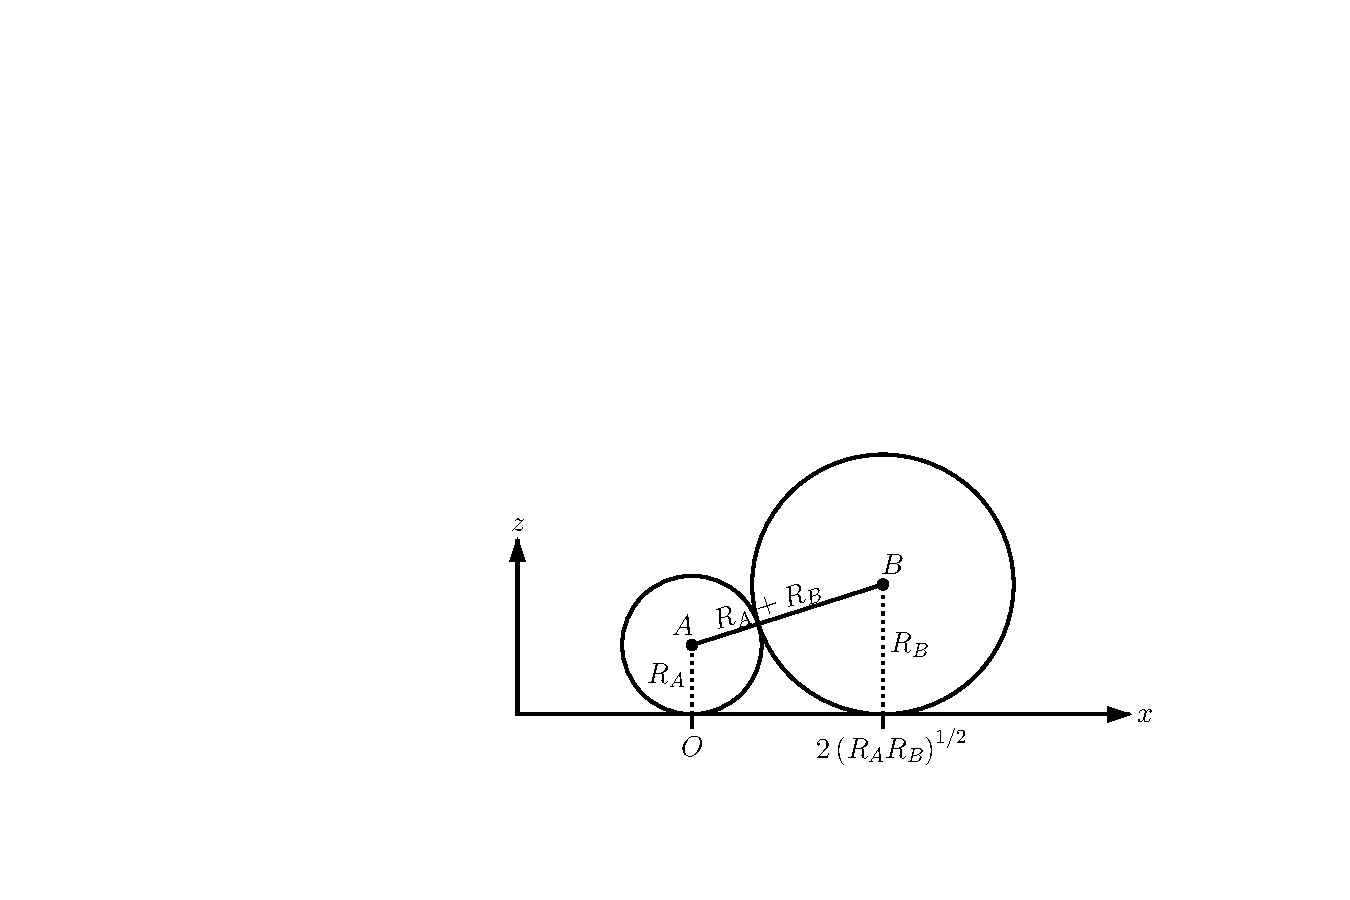
\includegraphics[width=10cm]{./figures/quasi2d/quasi2d_a.pdf}
     \caption{Quasi\--2D hard spheres can be modelled in 2D by using non\--additive interaction distances. Here two spheres sedimented on a plane have a contact distance given by twice the geometric mean of the radii.}
     \label{fig:nonadddemo}
\end{figure}

Since systems of colloidal monolayers can be treated as a 2D problem, this should enable them to be analysed with a 2D Voronoi diagram.
Voronoi analysis allows determination of the coordination environments around each particle, so that network properties such as the neighbour degree distribution and correlations can be calculated \cite{Earnshaw1994,Yang2002,Kumar2005,Chremos2007}.
This information can be used, for example, to give insights as to the phase behaviour in these systems \cite{Jaster1999,Pronk2004,Kapfer2015,Thorneywork2017}.
However, it is not initially clear how the non\--additivity will affect the calculation of the Voronoi diagram.
For instance, unlike a system of additive hard disks, it is not obvious if a unweighted or weighted variant of the Voronoi construction is most appropriate, and in the latter case what the weightings should be.
It will be demonstrated in the second half of this chapter that in fact the unweighted construction retains a precise physical meaning for \qtd{} systems, and is the natural choice for partitioning space in these monolayers.

\subsection{Experimental Analysis}

Raw experimental coordinates were kindly provided for a range of mono\-- and bidisperse colloidal systems by Thorneywork and Dullens \cite{Thorneywork2014,Thorneywork2017,alice2015a}.
The colloidal monolayers were prepared by dispersing particles of specific radii in a water\--ethanol mixture and sedimenting them on the base of a glass sample cell.
The samples were then imaged using an inverted bright-field microscope and particle coordinates obtained using standard particle tracking routines, to obtain raw particle coordinates.
Allowing a time of around $~10s$ between frames ensured that the particle positions are sufficiently decorrelated. 

\begin{table}
\centering
\caption{Summary of the experimental parameters which can be controlled in colloidal monolayers.}
\label{tab:expcolloidparams}
\begin{tabular}{@{}cccccc@{}}
\toprule
& \multicolumn{1}{c}{Mono} & \phantom{x} & \multicolumn{3}{c}{Binary} \\ 
\cmidrule{2-2} \cmidrule{4-6} 
& & & Large & Small & Total \\ 
\midrule
Radius & $R$ & & $R_l$ & $R_s$ & - \\
Radius ratio & 1 & & - & - & $\gamma=R_l/R_s$ \\
Composition & 1 & & $c_l$ & $c_s$ & 1 \\
Number density & $\rho$ & & $\rho_l=c_l\rho$ & $\rho_s=c_s\rho$ & $\rho=\rho_l+\rho_s$ \\
Packing fraction & $\phi=\rho\pi R^2$ & & $\phi_l=\rho_l\pi R_l^2$ & $\phi_s=\rho_s\pi R_s^2$ & $\phi=\phi_l+\phi_s$ \\
\bottomrule
\end{tabular}
\end{table}

Data was made available across a range of experimental conditions.
For the monodisperse systems, samples contained particles with radii of $R=1.395\mu$m, across a range of 2D packing fractions, $\phi$, as defined in equation \davidnote{ref}.
For bidisperse systems, which consist of two particle sizes, one ``large'' and the other ``small'', there are more free parameters to control, which are summarised in table \ref{tab:expcolloidparams}.
Firstly there is the radius ratio of the particles, $\gamma=R_l/R_s$ (the subscripts ``$l$'' and ``$s$'' will be used to denote variables corresponding to large and small particles respectively), which relates the relative particle sizes.
Secondly, the composition, $c_l$, $c_s$, determines the proportion of each particle type, where $c_l+c_s=1$.
Finally there is also the packing fraction, calculated with reference to one of the components $\phi_l$, $\phi_s$, or using all particles to give a total packing fraction $\phi=\phi_l+\phi_s$.
For completeness, it is noted that the composition can also be represented by $\phi_l/\phi$, but for the purposes of this work the definition above was found to be more intuitive.
The available experimental data contained systems at two radius ratios and a variety of compositions and packing fractions.
More specifically, these had either $R_s=1.395\mu$m and $R_l=3.05,2.02\mu$m, corresponding to size ratios of $\gamma=2.19, 1.45$ respectively.
In addition for each set of experimental conditions there were 100 configurations, which the exact compositions and packing fractions for each were determined and presented in table \ref{tab:expcolloid}

\begin{table}
\centering
\caption{Details of experimental colloidal samples. Samples are defined in terms of particle size dispersity, particle radius ratio, composition and total packing fraction. The mean value is supplied for each, with the standard deviation given in brackets.}
\label{tab:expcolloid}
\begin{tabular}{@{}ccccccccccc@{}}
\toprule
\multicolumn{1}{c}{Mono} & \phantom{x} & \multicolumn{2}{c}{Binary, $\gamma=2.19$} & \phantom{x} & \multicolumn{2}{c}{Binary, $\gamma=1.45$} & \phantom{x} & \multicolumn{2}{c}{Binary, $\gamma=1.45$}\\ 
\cmidrule{1-1} \cmidrule{3-4} \cmidrule{6-7} \cmidrule{9-10}
$\phi$ & & $c_l$ & $\phi$ &  & $c_l$ & $\phi$ & & $c_l$ & $\phi$  \\ 
\midrule
$0.655(1)$&&$0.201(1)$&$0.764(2)$&&$0.532(4)$&$0.571(1)$&&$0.233(1)$&$0.607(2)$\\
$0.616(1)$&&$0.182(1)$&$0.639(2)$&&$0.522(4)$&$0.477(4)$&&$0.208(1)$&$0.406(1)$\\
$0.509(1)$&&$0.192(2)$&$0.507(3)$&&$0.543(5)$&$0.267(1)$&&$0.226(3)$&$0.309(2)$\\
$0.427(1)$&&$0.189(2)$&$0.339(3)$&&$0.332(1)$&$0.629(1)$&&$0.091(1)$&$0.663(1)$\\
$0.341(1)$&&$0.187(7)$&$0.150(2)$&&$0.314(3)$&$0.499(3)$&&$0.107(1)$&$0.500(2)$\\
$0.289(0)$&& &&&$0.345(2)$&$0.337(2)$&&$0.087(1)$&$0.257(1)$\\
\bottomrule
\end{tabular}
\end{table}

The 2D experimental coordinates can be analysed using a Voronoi construction. An example for both a mono\-- and bidisperse configurations can be found in figure \ref{fig:expvoro}.
With the raw coordinates, the experimental samples can be treated analogously to configurations generated from computation.
The only difference is that the experimental images are by nature aperiodic, and so when analysing the network properties of the Voronoi diagram, the cells close to the boundary must be neglected, to remove any edge effects. 
However, careful examination of figure \ref{fig:expvoro1} reveals some small imperfections in the data, as there are instances where the monodisperse particles appear to overlap.
This is not a result of differences in particle size, but rather the presence of ``phantom'' particles deriving from the imaging process.
Extracting particle positions from the experimental data is highly non\--trivial, in particular removing points arising from interstitial sites between densely packed particles \cite{alice2015a}.
Whilst this becomes more problematic at higher packing fractions, they are however still few and far between.
It should also be point out here that the tracking routines are able to detect the difference between large and small particles in bidisperse systems, allowing Voronoi cells to be associated to particles of a specific size.
The actual results of the analysis of these experimental systems will be discussed alongside the results from computation in section \davidnote{ref}.

\begin{figure}[bt]
     \centering
     
      \begin{subfigure}[b]{0.48\textwidth}
         \centering
         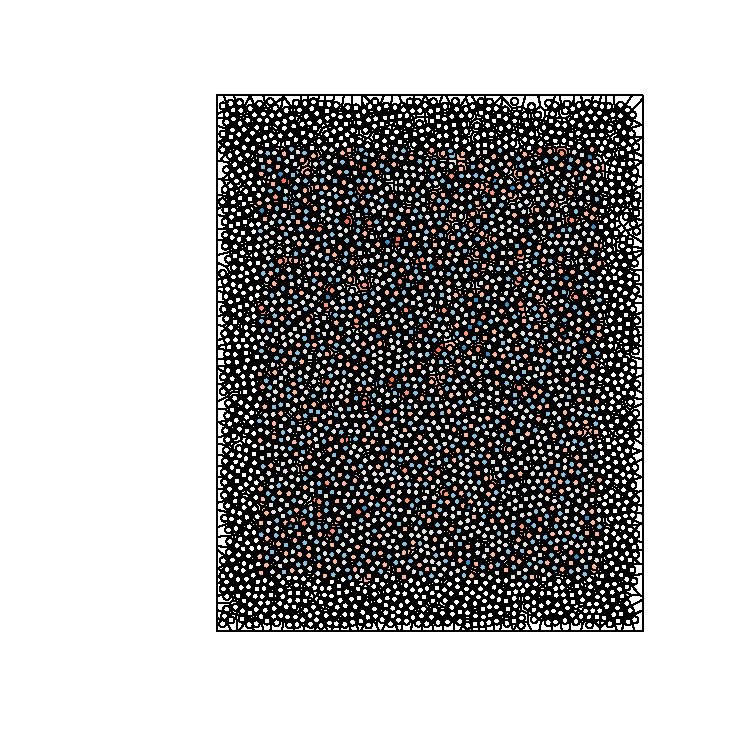
\includegraphics[width=\textwidth]{./figures/quasi2d/exp_mono.pdf}
         \caption{Mono, $\phi=0.509$}
         \label{fig:expvoro1}
     \end{subfigure}
     \hfill
       \begin{subfigure}[b]{0.48\textwidth}
         \centering
         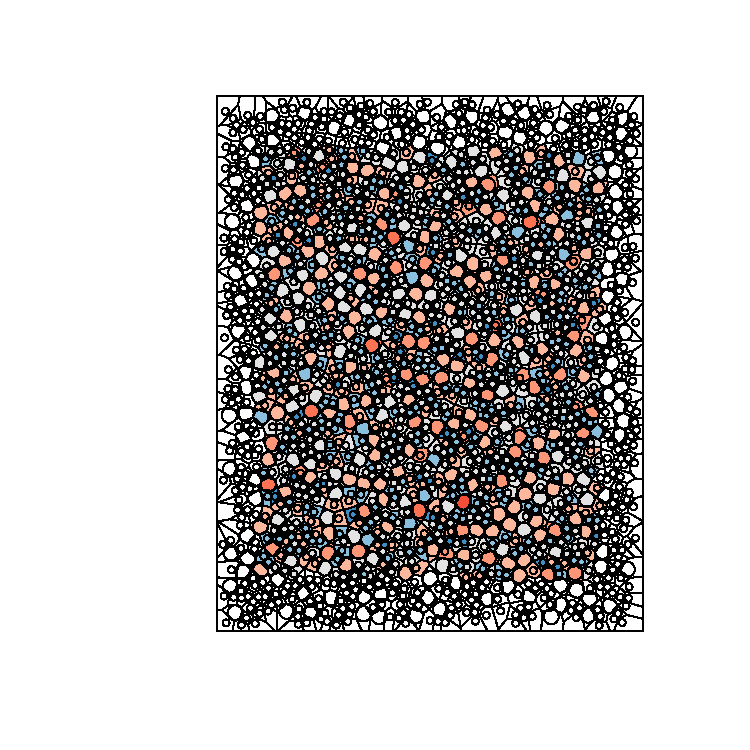
\includegraphics[width=\textwidth]{./figures/quasi2d/exp_lsr.pdf}
         \caption{Binary, $\gamma=2.19$, $c_l=0.192$, $\phi=0.507$}
         \label{fig:expvoro2}
     \end{subfigure}
     \hfill
     
     \caption{Voronoi analysis of two example experimental snapshots, of a monodisperse and bidisperse \qtd{} colloidal monolayer (system parameters in captions).}
     \label{fig:expvoro}
\end{figure}

\subsection{Non\--additive Hard Disk Monte Carlo}

Experimental data can be compared and contrasted with configurations generated from simulation.
Hard particle \mc{} was introduced in section \ref{s:hardparticlemc} as a method to generate such configurations computationally.
One could set up a 3D system of hard spheres constrained to a plane, but as discussed above it is preferable to employ a non\--additive hard disk model.
In this modification, if two particles are separated by a distance, $r_ij$, the pair potential is:
\begin{equation}
	\mathcal{U}_{ij} = \begin{cases} \infty \quad &r_{ij}<2\left(R_iR_j\right)^{1/2} \\ 0 \quad &\text{otherwise} \end{cases}\,.
\end{equation}
The remainder of the algorithm proceeds the same as in section \ref{s:hardparticlemc}.


\section{Monodisperse Spheres}

\davidnote{link to generalised earlier}

\begin{figure}[bt]
     \centering
     
      \begin{subfigure}[b]{0.45\textwidth}
         \centering
         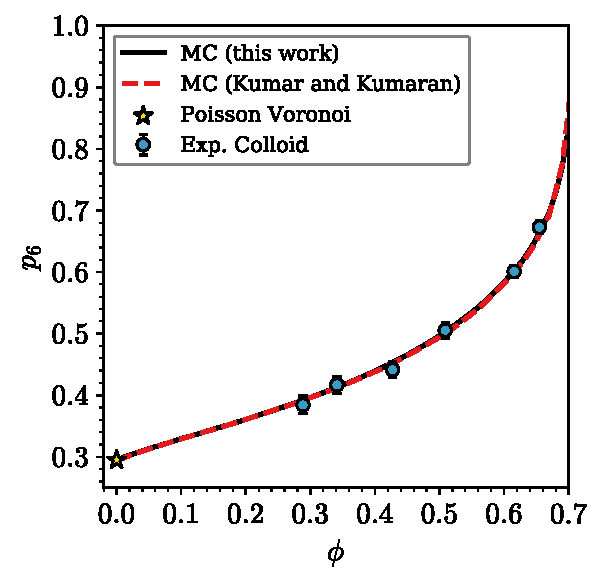
\includegraphics[height=7cm]{./figures/quasi2d/mono_phi_p6.pdf}
         \caption{}
         \label{fig:mono1}
     \end{subfigure}
     \hfill
       \begin{subfigure}[b]{0.45\textwidth}
         \centering
         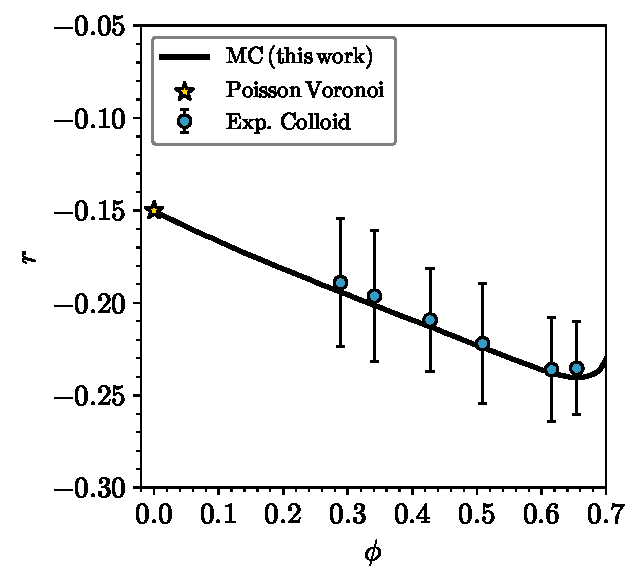
\includegraphics[height=7cm]{./figures/quasi2d/mono_phi_r.pdf}
         \caption{}
         \label{fig:mono2}
     \end{subfigure}
     \hfill
    
     \caption{Network properties of monodisperse systems of \qtd{} hard spheres, in terms of the proportion of hexagons, panel (a), and the assortativity, panel (b). Data is presented both from simulation and experiment, with the experimental points indicating the mean value and two standard deviations either side. A comparison is also made in panel (a) to a previous study \cite{Kumar2005}, to which there is excellent agreement.}
     \label{fig:mono}
\end{figure}


\subsection{Network Properties}

\section{Bidisperse Spheres}

\begin{figure}[bt]
     \centering
     
      \begin{subfigure}[b]{0.45\textwidth}
         \centering
         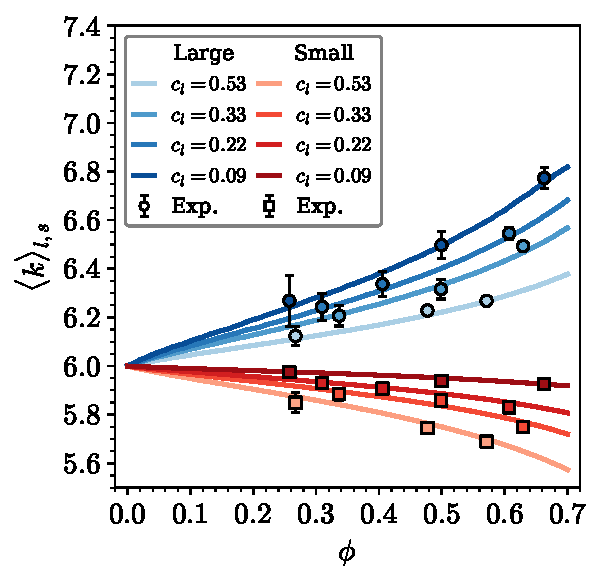
\includegraphics[height=7cm]{./figures/quasi2d/bi_ssr_phi_k.pdf}
         \caption{}
         \label{fig:bi1}
     \end{subfigure}
     \hfill
      \begin{subfigure}[b]{0.45\textwidth}
         \centering
         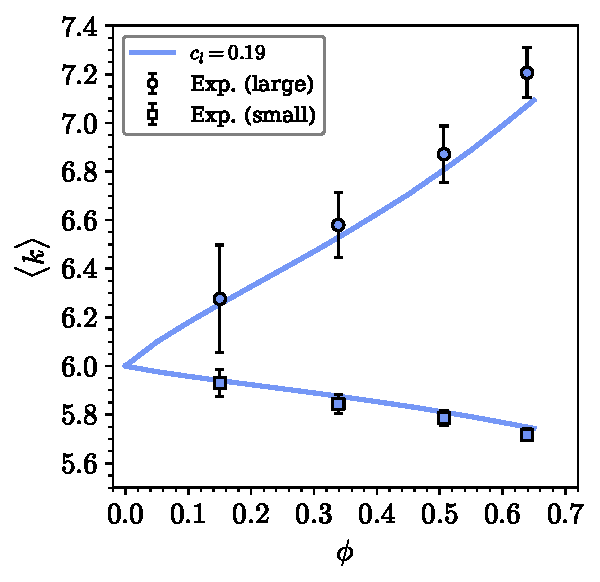
\includegraphics[height=7cm]{./figures/quasi2d/bi_lsr_phi_k.pdf}
         \caption{}
         \label{fig:bi2}
     \end{subfigure}
     \hfill
     
      \begin{subfigure}[b]{0.45\textwidth}
         \centering
         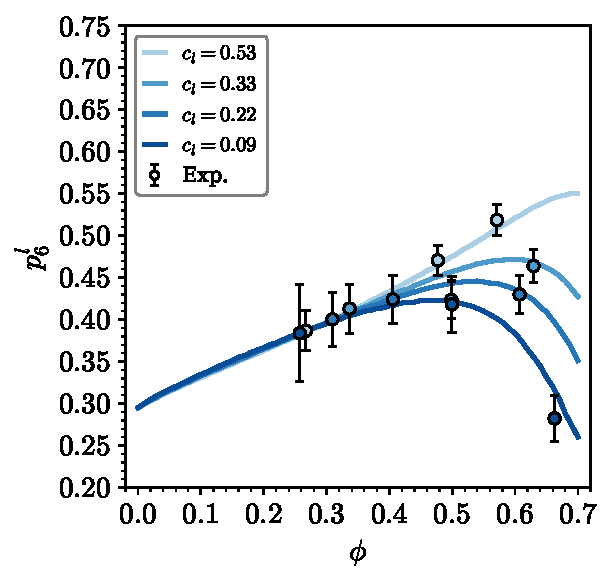
\includegraphics[height=7cm]{./figures/quasi2d/bi_ssr_l_phi_p6.pdf}
         \caption{}
         \label{fig:bi3}
     \end{subfigure}
     \hfill
     \begin{subfigure}[b]{0.45\textwidth}
         \centering
         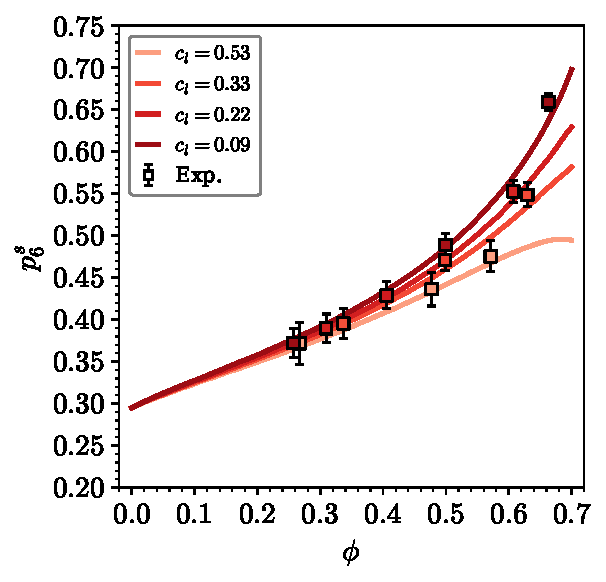
\includegraphics[height=7cm]{./figures/quasi2d/bi_ssr_s_phi_p6.pdf}
         \caption{}
         \label{fig:bi3}
     \end{subfigure}
     \hfill
    
     \caption{xxx}
     \label{fig:mono}
\end{figure}

\subsection{Network Properties}

%The case of \qtd{} polydisperse spheres is a generalisation of the mono\-- and bidisperse systems discussed already in this chapter.
%Owing to this generality, a different approach will be taken in this section, and the meaning of the Voronoi diagram carefully examined in the context of \qtd{} hard sphere systems.
%XXX

\section{Voronoi Diagrams in Quasi\--2D Systems}

\subsection{Stereological Relationships}
\label{sec:vorrel}

When studying quasi\--2D colloids, it is possible to construct a 3D weighted Voronoi using the coordinates of the particle centres, $c_i=\left(x_i,y_i,\rs_i\right)$.
However, in most cases researchers prefer to analyse configurations using a 2D Voronoi using the projected particle centres $c_i^\prime=\left(x_i,y_i\right)$. 
The rational behind this is clear: 2D analysis is easier to visualise and rationalise.
In addition, as in figure \ref{fig:main}(a), for monodisperse systems the 3D representation contains no more information on neighbouring interactions and assigned volumes than the 2D analogue.
However, as in figure \ref{fig:main}(c), for polydisperse particles whilst this may be a good first approximation, this is not necessarily accurate, and so it is important to examine the relationship between Voronoi diagrams in two and three dimensions to ensure correct physical meaning is attributed to the Voronoi analysis.

\subsubsection{Limiting Case with Basal Plane}

We first consider the stereological relationship between the 3D weighted Voronoi and the 2D tessellation formed from the intersection of the radical planes with the basal tangent plane.
In figure \ref{fig:main}(c), this corresponds to the bottommost 2D tessellation.
To do this take the arrangement in figure \ref{fig:geometry}(a), with two spheres $A$,$B$ separated by the dividing radical plane, $V$, and sharing the tangent plane, $T$, with equation $z=0$.
The distance between the sphere centres is $d_{AB}$, whilst the distance between the projected centres is denoted $d_{AB}^\prime$.
The dividing plane $V$, has a normal given by $\mathbf{n} =\overrightarrow{AB}=d_{AB}^\prime\boldsymbol{\hat{\textbf{\i}}}+\left(\rs_B-\rs_A\right)\mathbf{\hat{k}}$.
In addition the point $D$ which lies on $V$ is located at $\overrightarrow{OD}=d_{A}\mathbf{\hat{n}}+\rs_A\mathbf{\hat{k}}$ where $d_{A}=\frac{\rs_A^2-\rs_B^2+d_{AB}^2}{2d_{AB}}$ and $\abs{\mathbf{n}}=d_{AB}$.
Defining the direction of $x$ as as the projection of $d_A\mathbf{\hat{n}}$ on the basal plane, the plane equation for $V$ can be deduced as:
\begin{equation}
	\label{eq:plane}
	d_{AB}^\prime x+\left(\rs_B-\rs_A\right)z=\frac{\left(d_{AB}^\prime\right)^2}{2}.
\end{equation}
The intersection of $V$ with $T$ occurs at $z=0$, and so we find that line of intersection is given simply by $x=d_{AB}^\prime/2$.
However we notice something interesting about this result.
This dividing line in 2D is the same as that which would be obtained from constructing the 2D unweighted Voronoi using the projected particle centres $c^\prime_i$.
As this must be true for all pairs of neighbouring particles, it follows that the entire 2D unweighted Voronoi will be constructed. 
This leads to the key relationship of this work: the unweighted 2D Voronoi diagram constructed from the projected particle centres is topologically equivalent to the tessellation formed by taking the basal faces of the polyhedra in the weighted 3D Voronoi diagram.

\begin{figure*}
	\includegraphics[width=\textwidth]{./figures/figure_2.png}
	\caption{Panel (a) shows two spheres and the dividing radical plane between them. The radical plane intersects the tangent plane at half the horizontal distance between the particles. This intersection generates the same dividing line in the tangent plane as would the unweighted Voronoi using the projected particle positions.
Panel (b) shows three spheres and the 3D weighted Voronoi polyhedron formed around sphere $A$. The height of the cell is given by the topmost point, denoted $h_S\left(R_A\right)$. Panel (c) shows the same three spheres and the polyhedron that would be formed from stacking 2D Voronoi tessellations with disk radii as weights. As the weight for $A$ is not defined above the sphere diameter, the polyhedron is truncated in comparison with in panel (b). The height of the cell is then given by $h_D\left(R_A\right)=2R_A$.}
	\label{fig:geometry}
\end{figure*}

\subsubsection{General Case with Arbitrary Horizontal Plane}

Taking the basal faces of the 3D Voronoi polyhedra can equally be thought of as taking a horizontal cut through the tessellation at $z=0$.
The result above is essentially a special case of the fact that a cut through a 3D Voronoi must yield a tessellation which is equivalent to some weighted 2D Voronoi\cite{Imai1985,Rivier1990}.
Following from the result above, we may ask what is the analogous relationship between a 2D and 3D Voronoi when taking a cut at arbitrary $z$, as in figure \ref{fig:main}(c).
Revisiting the simple arrangement in figure \ref{fig:geometry}(a),
for a given horizontal cut height, $z$, we now define the projected particle centres as $c_i^\prime=\left(x_i,y_i,z\right)$.
Regardless of the the value of $z$, we note that the distances between the projected centres remain the same at $d_{AB}^\prime$.
To obtain the same distance between the projected particle centres and the dividing plane using both a 2D and 3D Voronoi, it can be seen from combining equations \eqref{eq:rad} and \eqref{eq:plane} that:
\begin{equation}
	\label{eq:condition}
	w_A^2-2\rs_Az = w_B^2-2\rs_Bz.
\end{equation}
The simplest solution for the weights that satisfy this equation is therefore:
\begin{equation}
	\label{eq:mapweights}
	w_{S,i} = \left(2\rs_iz\right)^{1/2}.
\end{equation}
Again as this will naturally extend to a collection of many particles, we obtain a more general relationship: the tessellation formed from a horizontal cut through a 3D weighted Voronoi diagram is topologically equivalent to the 2D Voronoi diagram calculated from the projected particle centres, weighted according to equation \eqref{eq:mapweights}.
Indeed, we see that the first result is simply a limiting case of this second result, where $z=0$ and the weights are trivially zero.
We shall refer to this 2D weighted Voronoi diagram as the sphere\--weighted Voronoi and denote variables associated with it with a subscript $S$.

\subsubsection{Connection to System of Hard Disks}

A horizontal cut through a 3D system of hard spheres will produce a 2D system of hard disks.
The radii of these disks will be related to the radii of the spheres, and if they are used as weights in a 2D Voronoi analysis they will also satisfy equation \eqref{eq:condition}:
\begin{equation}
	\label{eq:radii}
	w_{D,i}  = \left(2\rs_i z-z^2\right)^{1/2}.
\end{equation}
This suggests that the tessellation formed from the horizontal cut through the 3D Voronoi should also be equivalent to the 2D Voronoi using these disk radii.

However, there is a caveat to this result. 
It is clear that equation \eqref{eq:radii} is only well defined for $z\leq 2\rs_i$ \ie{} the cut height is less than the sphere diameter.
There is no such constraint for the polyhedral cells in the 3D weighted Voronoi, which may readily extend above the associated particle.
Therefore, the result above is only strictly true when the cut height is less than the smallest sphere diameter.
A modification is made where points which have diameters less than the cut height are excluded from the 2D calculation.
These excluded particles will therefore not have cells in the Voronoi tessellation.
In this case some 3D cells will become truncated in the 2D representation, as shown in figures \ref{fig:geometry}(b) and \ref{fig:geometry}(c).
This will lead to an increasing difference between the two types of partitions as the cut height is increased, as demonstrated in figure \ref{fig:vorocomp}.
This 2D weighted diagram we shall refer to as the disk\--weighted Voronoi and denote variables associated with it with a subscript $D$.

\begin{figure}
	\includegraphics[width=7cm]{./figures/figure_3.pdf}
	\caption{Comparison of the tessellations formed from a horizontal cut through a 3D Voronoi diagram weighted by sphere radii (a) and a 2D Voronoi diagram weighted by disk radii (b), where indices (i)\--(iv) indicate increasing $z$ values.
	The same configuration is used as in figure \ref{fig:main}, with the horizontal cuts corresponding to the left hand diagrams.
	Black circles indicate the particle radii at the cut height, which also correspond to the weights in the disk\--weighted Voronoi. Black points indicate the projected particle centres, whilst grey points indicate particles without corresponding cells in the 2D tessellaion.}
	\label{fig:vorocomp}
\end{figure}

\subsection{Properties of Voronoi Tessellations}

We will discuss important properties of the sphere and disk\--weighted Voronoi diagrams which will aid with their analyses.
These include the expected number of points at a given cut height, the weight distribution of the included points and the nearest\--neighbour distances between them.
We note that these are the quantities that appear in equation \eqref{eq:rad} and therefore govern the wider properties of the Voronoi diagram. 
We will show the analytic results for our model of lognormally distributed sphere radii, but the results extend to any configuration where the sphere radii are known.

\subsubsection{Average Nearest\--Neighbour Distances}

A useful metric is the expected distance between points in a Voronoi diagram at different cut heights, as this can be used to rationalise much of the observed behaviour.
In order to do this we will assume that particles are uniformly distributed (the ideal gas), neglecting the short range liquid structure.
Whilst this might seem an over\--simplification, not only does the approximation get better at lower packing fractions but also as the cut height is increased, particles are lost from the tessellation and their positions become effectively decorrelated. 

First we wish to find the average distance between all points in neighbouring Voronoi cells at a given cut height, $\ed$.
We introduce the number density at a given cut height, denoted $\rho_z$. 
This will be the number of points at height $z$, divided by the total area of the 2D Voronoi diagram.
It can therefore be expressed:
\begin{equation}
	\label{eq:numden}
	\rho_z = \rho_0 \zN,
\end{equation}
where $\rho_0$ is the number density considering all points (as must be the case at $z=0$), and $N\left(z\right)$ is the proportion of particles included at a given cut height.
By dividing the area equally between all particles, we expect the average distance between neighbouring points in the 2D Voronoi diagram to follow:
\begin{equation}
	\label{eq:ndist}
	\ed = 2\left(\frac{1}{\pi\rho_z}\right)^{1/2}.%=2\left(\frac{1}{\pi\rho_0\zN}\right)^{1/2}.
\end{equation}

Alternatively, we can opt to find the average distance to the $n^{\mathrm{th}}$ nearest neighbour, $\edn$.
If again a uniform distribution of spheres is assumed (\ie{} the dilute limit), equation (12) of Bhattacharyya and Chakrabarti\cite{Bhattacharyya2008}, shows that in two dimensions, this is given by the equation:
\begin{equation}
	\label{eq:nndist}
	\edn = \left(\frac{1}{\pi\rho_z}\right)^{1/2}\frac{\Gamma{\left(n+1/2\right)}}{\Gamma{\left(n\right)}}.
\end{equation}
%which again assumes a uniform distribution of points.

\subsubsection{Properties of Disk\--Weighted Voronoi}

The properties of the disk\--weighted Voronoi are somewhat easier to see and so we begin with these.
The height below which a Voronoi cell is defined for a particle of a certain radius is given exactly by $h_D\left(R\right)=2R$, as in figure \ref{fig:geometry}(c).
Hence, for a given cut height, the particles with associated cells in the tessellation will be all those with radii in excess of the inverse function $h_D^{-1}\left(z\right)=z/2$.
The proportion of particles with associated cells above a given cut height, denoted $\nDz$, is therefore simply related to the cumulative distribution function of the sphere radii:
\begin{equation}
	\label{eq:ndz}
	\nDz = \int_{z/2}^\infty f\left(\rs\right) \dd\rs = \frac{1}{2}\text{erfc}\left[\frac{\ln{\left(z/2\right)}-\mu}{\sqrt{2\sigma^2}}\right],
\end{equation}
as all particles with $R < z/2$ are neglected.

%The probability distribution of weights for the points which remain, $\gDwz$, can be found by substitution of variables, using equations \eqref{eq:radii} and \eqref{eq:lognormal},
%\begin{equation}
%	\gDwz = \frac{\wD}{z\nDz}f\left(\frac{\wD^2+z^2}{2z}\right).
%\end{equation}
The moments of the weight distribution function at a given cut height can then be calculated by integrating over the range of the remaining particle radii,
\begin{equation}
	\label{eq:wmom}
	\ewDn = \frac{1}{\nDz}\int_{z/2}^\infty  \left(2Rz-z^2\right)^{n/2} f\left(R\right) \dd R.
\end{equation}
as required.
For example, the analytic solution for the second moment can be found in section \ref{sec:packingfrac}.
%\begin{align}
%	\label{eq:pfw}
%	\ewDii &= \int_{0}^\infty  \frac{\wD^3}{z\nDz} f\left(\frac{\wD^2+z^2}{2z}\right) \dd\wD \nonumber \\
%	%&= \frac{z}{\nDz}\exp{\left(\mu+\frac{\sigma^2}{2}\right)}\text{erfc}\left[\frac{\ln{\left(z/2\right)}-\mu-\sigma^2}{\sqrt{2\sigma^2}}\right]+\nonumber \\ &\phantom{=} -\frac{z^2}{2\nDz}\text{erfc}\left[\frac{\ln{\left(z/2\right)}-\mu}{\sqrt{2\sigma^2}}\right] \nonumber \\
%	&= 2\langle \rs\rangle z\frac{N_D\left(ze^{-\sigma^2}\right)}{\nDz}-z^2.
%\end{align}
%\begin{align}
%	\label{eq:wiid}
%	\ewDii &= \frac{1}{\nDz}\int_{z/2}^\infty  \left(2Rz-z^2\right) f\left(R\right) \dd R \nonumber \\
%	&= 2\langle \rs\rangle z\frac{N_D\left(ze^{-\sigma^2}\right)}{\nDz}-z^2.
%\end{align}

%We note the pleasing similarity between this result and equation \eqref{eq:radii}, and see that there will be parity when $\sigma=0$ \ie{} the monodisperse limit. 
%For finite $\sigma$, as the function \eqref{eq:ndz} is monotonically decreasing, the ratio of the normalising functions acts to increase the second moment of the weights as would be expected by removing the smaller particles from the system first.

\subsubsection{Properties of Sphere\--Weighted Voronoi}

For the sphere\--weighted Voronoi, the maximum height of the Voronoi cell for a particle of a certain radius, $h_S\left(R\right)$, is not precisely defined with $R$.
We will derive an approximate form below, but first note that regardless of the functional form of $h_S\left(R\right)$, in a similar manner to above we can write an equation for the proportion of particles with associated cells above a given cut height, denoted $\nSz$, as:
\begin{equation}
	\label{eq:nsz}
	\nSz = \int_{h_{S}^{-1}\left(z\right)}^\infty f\left(\rs\right) \dd\rs = \frac{1}{2}\text{erfc}\left[\frac{\ln{\left(h_{S}^{-1}\left(z\right)\right)}-\mu}{\sqrt{2\sigma^2}}\right],
\end{equation}
with the moments of the weights at a given cut height provided by:
%\begin{align}
%	\label{eq:wiis}
%	\ewSii &= \frac{1}{\nSz}\int_{\hz}^\infty  2Rz f\left(R\right) \dd R \nonumber \\
%	&= 2\langle \rs\rangle z\frac{N_S\left(ze^{-\sigma^2}\right)}{\nSz}.
%\end{align}
\begin{equation}
	\label{eq:wns}
	\ewSn = \frac{1}{\nSz}\int_{h_{S}^{-1}}^\infty  \left(2Rz\right)^{n/2} f\left(R\right) \dd R,
\end{equation}
in analogy with the disk\--weighted case.

We now discuss the functional form of $h_S\left(R\right)$.
Rather than an exact relationship, we wish to find the expected Voronoi cell height for a given particle radius.
The height of a Voronoi cell is a complex function that must depend on both the radius of the associated particle and the distances to neighbouring particles. 
In the following arguments it will be useful to refer to figures \ref{fig:main}, \ref{fig:geometry} and \ref{fig:vorocomp}.
Consider a reference particle of a given radius, $R^\prime$.
Crucially, the dividing planes forming the Voronoi polyhedron around it will only converge to a point when the neighbouring particles are larger than the reference particle.
For the purposes of this analysis, we can therefore think of the particle operating in a reduced density system containing only the particles with radii greater of equal to the reference particle.
The density is therefore,
\begin{equation}
	\label{eq:rhoref}
	\rho^\prime = \rho_0 \int_{R^\prime}^{\infty} f\left(R\right) \dd R,
\end{equation}
and mean average particle radius,
\begin{equation}
	\langle R^\prime \rangle = \frac{\int_{R^\prime}^{\infty} R f\left(R\right) \dd R }{\int_{R^\prime}^{\infty} f\left(R\right) \dd R}.
\end{equation}
In addition, the average $n^{\mathrm{th}}$ nearest neighbour distance will be given by equation \eqref{eq:nndist}, substituting the density from equation \eqref{eq:rhoref} above.

We therefore consider the average environment around the reference particle to consist of particles with radii $\langle R^\prime \rangle$ at located at successive distances $\langle d^\prime_n\rangle$.
These particles will generate dividing Voronoi planes according to equation \eqref{eq:plane}.
If we then assume that on average the highest point in the Voronoi polyhedron will occur above the particle centre (\ie{} $x=0$, see for example the cells in figure \ref{fig:main}), we find:
\begin{equation}
	h_{S,n}\left(R^\prime\right) \sim \frac{\langle d^\prime_n\rangle^2}{2\left(\langle R^\prime \rangle - R^\prime\right)}.
\end{equation}
These can be averaged over $m$ nearest neighbours to give the result:
\begin{equation}
	h_S\left(R^\prime\right) = \frac{1}{2m\left(\langle R^\prime\rangle-R^\prime\right)}\sum\limits_{n=1}^{m} \langle d^\prime_n \rangle^2.
\end{equation} 
As will be shown in section \ref{sec:numres} and figure \ref{fig:nphi}, we  found that averaging over $m=3$ nearest neighbour distances gave a good fit to the observed numerical distribution.
We rationalise this on the basis that the top vertex is formed from the intersection of three neighbouring planes, which originate from the closest three particles.

The important thing about this functional form is that the expected height of the Voronoi cell scales quickly with particle radius, unlike in the disk\--weighted case.
This is a result of the density of larger particles decreasing quickly with particle size, such that the average interaction distances become increasingly long and the radical planes approach vertical.

\subsection{Packing Fraction}
\label{sec:packingfrac}

One complication with quasi\--2D hard spheres is that the definition of packing fraction is ambiguous.
The 2D packing fraction, $\phi_{2D}$, is usually defined as
\begin{equation}
	\label{eq:simplepackingfrac}
	\phi_{2D}=\pi\rho\langle \rs^2\rangle
\end{equation}
where $\rho$ is the number density.
For a quasi\--2D system this definition is not rigorous, as it can lead to a packing fraction greater than unity.

As an example, consider the binary crystalline lattice in figure \ref{fig:crystalpackingfrac}, consisting of a two particle types with radius ratio $\gamma$.
At $\gamma=0$ the lattice is the hexagonal close packed structure which has the well known maximal monodisperse packing limit of $\frac{\pi}{2\sqrt{3}}\approx0.907$.
As $\gamma$ increases, the smaller particles swell in the tetrahedral holes without affecting the large particle positions, and so the na\"ive \td{} packing fraction rises, peaking at $\frac{11\pi}{18\sqrt{3}}\approx1.108$ when $\gamma=\frac{1}{3}$ (the contact distance).
Beyond this radius ratio the small particles can no longer be accommodated in the tetrahedral holes, and so the larger particles are forced apart which leads to a an initial decrease in packing fraction before the hexagonal close packed limit is approached once more.
We see that over this range the packing fraction exceeds unity and therefore obscures the physical meaning.

Moving to 3D does not necessarily solve the issue, as it is now not clear what volume (and therefore number density) is most appropriate.
%This problem is exacerbated as the polydispersity in the system increases.
However, considering quasi\--2D packings as a series of stacked sections through the 3D system allows an alternative definition of packing fraction:
\begin{equation}
	\label{eq:packingfrac}
	\zphi = \pi\rho_z\ewDii,
\end{equation}
as a function of $z$, the horizontal cut height, where $\rho_z$ and $\ewDii$ are provided by equations \eqref{eq:numden} and \eqref{eq:wmom} respectively.
The rationale for this equation is as follows. 
As the value, $\ewDii$, measures the average square radius of the circular sections in a cut of given height; here $\zphi$ quantifies the proportion of the total area occupied by the particle sections in the cut plane.

We propose that the overall packing fraction could thereby by quantified in these systems by $\text{max}\left[\phi\left(z\right)\right]$.
Referring again to figure \ref{fig:crystalpackingfrac}, we see that this definition gives values for the packing fraction which are now consistent with intuition.
For the region where $\gamma\leq\frac{1}{3}$ and the large particle lattice is unperturbed by the small particles, the maximal monodisperse packing limit is found.
Again beyond this the packing fraction then drops as the smaller particles swell above the contact distance before the hexagonal close packed lattice is once again recovered.
In addition, if this definition were applied to the simpler systems in figures \ref{fig:main}(a),(b), it would match with packing fraction calculated using the disks of the same radii as the spheres. 

\begin{figure}[bt]
	\includegraphics[width=8cm]{./figures/figure_4.png}
	\caption{Variation in packing fraction for a binary crystal with varying radius ratio, $\gamma$.
	Using the standard 2D packing fraction leads to values greater than unity whereas taking the maximum packing fraction with cut height limits the packing fraction to the known maximal packing limit.}
	\label{fig:crystalpackingfrac}
\end{figure}

For a polydisperse system, the explicit form of the second moment for the lognormal distribution can be calculated as,
\begin{align}
	\label{eq:wiid}
	\ewDii &= \frac{1}{\nDz}\int_{z/2}^\infty  \left(2Rz-z^2\right) f\left(R\right) \dd R \nonumber \\
	&= 2\langle \rs\rangle z\frac{N_D\left(ze^{-\sigma^2}\right)}{\nDz}-z^2.
\end{align}
We note the pleasing similarity between this result and equation \eqref{eq:radii}, and see that there will be parity when $\sigma=0$ \ie{} the monodisperse limit. 
Intuitively, the form of the packing fraction with $z$ and its maximal value is independent of the number density and is instead solely a property of the sphere radii distribution. 

\section{Polydisperse Spheres}

\subsection{Network Properties}

\section{Chapter Summary}